
%--- 目录 ---
\begin{frame}{目录}
  \begin{itemize}
    \item 什么是图像分类?
    \item 我们如何改进图像分类?(数据增强)
    \item 真实案例:灾害图像
    \item 项目:AI生成的图像能帮忙吗?
  \end{itemize}
\end{frame}

% \begin{refsection}
%   \begin{frame}
%     \centering
%     \vspace{2.5cm}
%     {\LARGE \textbf{图像分类简介}\\[0.5em]
%     \textbf{基于深度学习}}
%   \end{frame}
% \end{refsection}


\begin{frame}{什么是图像分类?}
  \begin{itemize}
    \item 计算机学习识别图片中的内容(如猫、狗、飞机等)。
    \item 我们用大量带标签的图片来教计算机。
    \item 目标:为新图片预测正确的标签。
  \end{itemize}
  \centering
  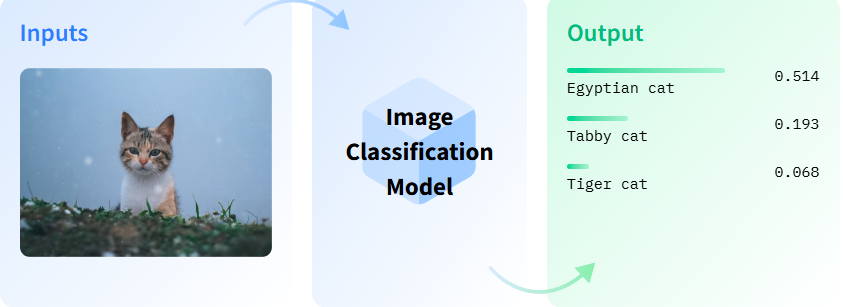
\includegraphics[height=0.6\textheight]{image_classification_idea.png}
\end{frame}

%--- 它是如何工作的? ---
\begin{refsection}
  \begin{frame}{它是如何工作的?}
    \begin{flushleft}
    神经网络是一种特殊的计算机程序,可以从大量示例图片中学习模式。随着时间推移,它们在区分图片方面会变得越来越好。
    \end{flushleft}
    \begin{figure}
      \begin{minipage}{0.48\linewidth}
        \centering
        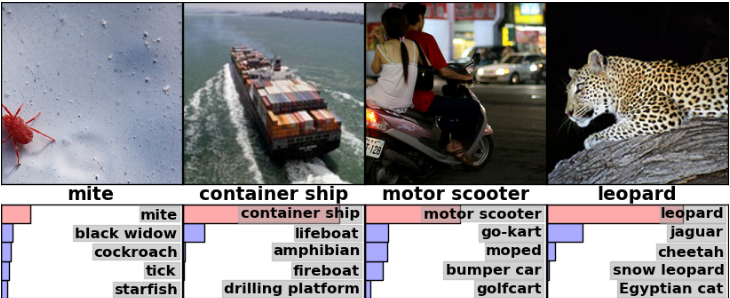
\includegraphics[width=0.95\linewidth]{imagenet2.png}
        \caption[]{\scriptsize ILSVRC-2010~\parencite{imagenet2010challenge}测试图片及模型认为最可能的五个标签~\parencite{krizhevskyImageNetClassificationDeep2012}。}
      \end{minipage}%
      \hfill
      \begin{minipage}{0.48\linewidth}
        \centering
        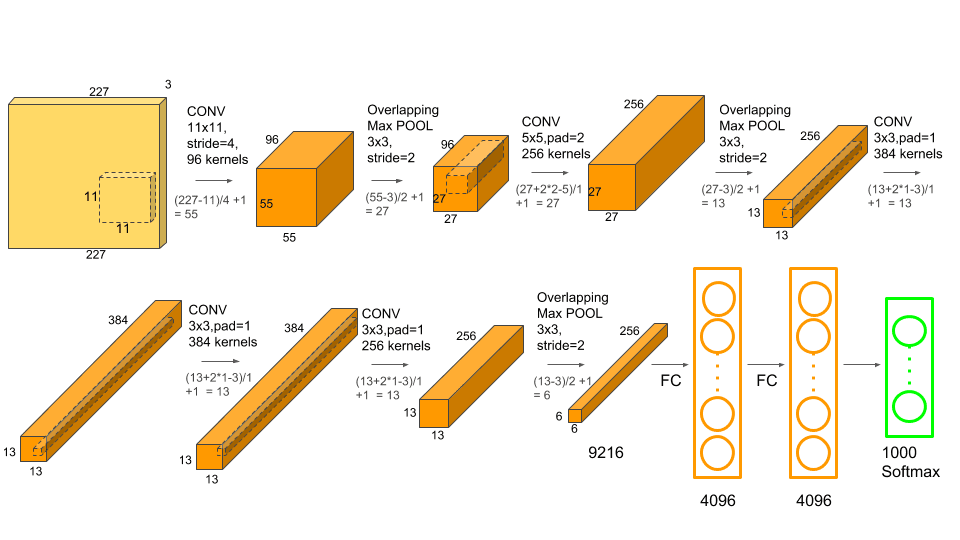
\includegraphics[width=0.95\linewidth]{alexnet.png}
        \caption[]{\scriptsize 图像分类神经网络示例:AlexNet~\parencite{krizhevskyImageNetClassificationDeep2012}。}
      \end{minipage}
    \end{figure}
    \bottomleftrefs
  \end{frame}
  \end{refsection}



%--- 现代模型:CLIP ---
\begin{refsection}
\begin{frame}{现代模型:CLIP}
  % \vspace{-0.7em}
  \begin{itemize}
    \item CLIP学习将图片和文本进行匹配。
    \item 它可以通过理解描述来识别新事物。
    \item 不仅仅用于分类,还适用于多种任务。
  \end{itemize}
  \centering
  \begin{figure}
    \centering
    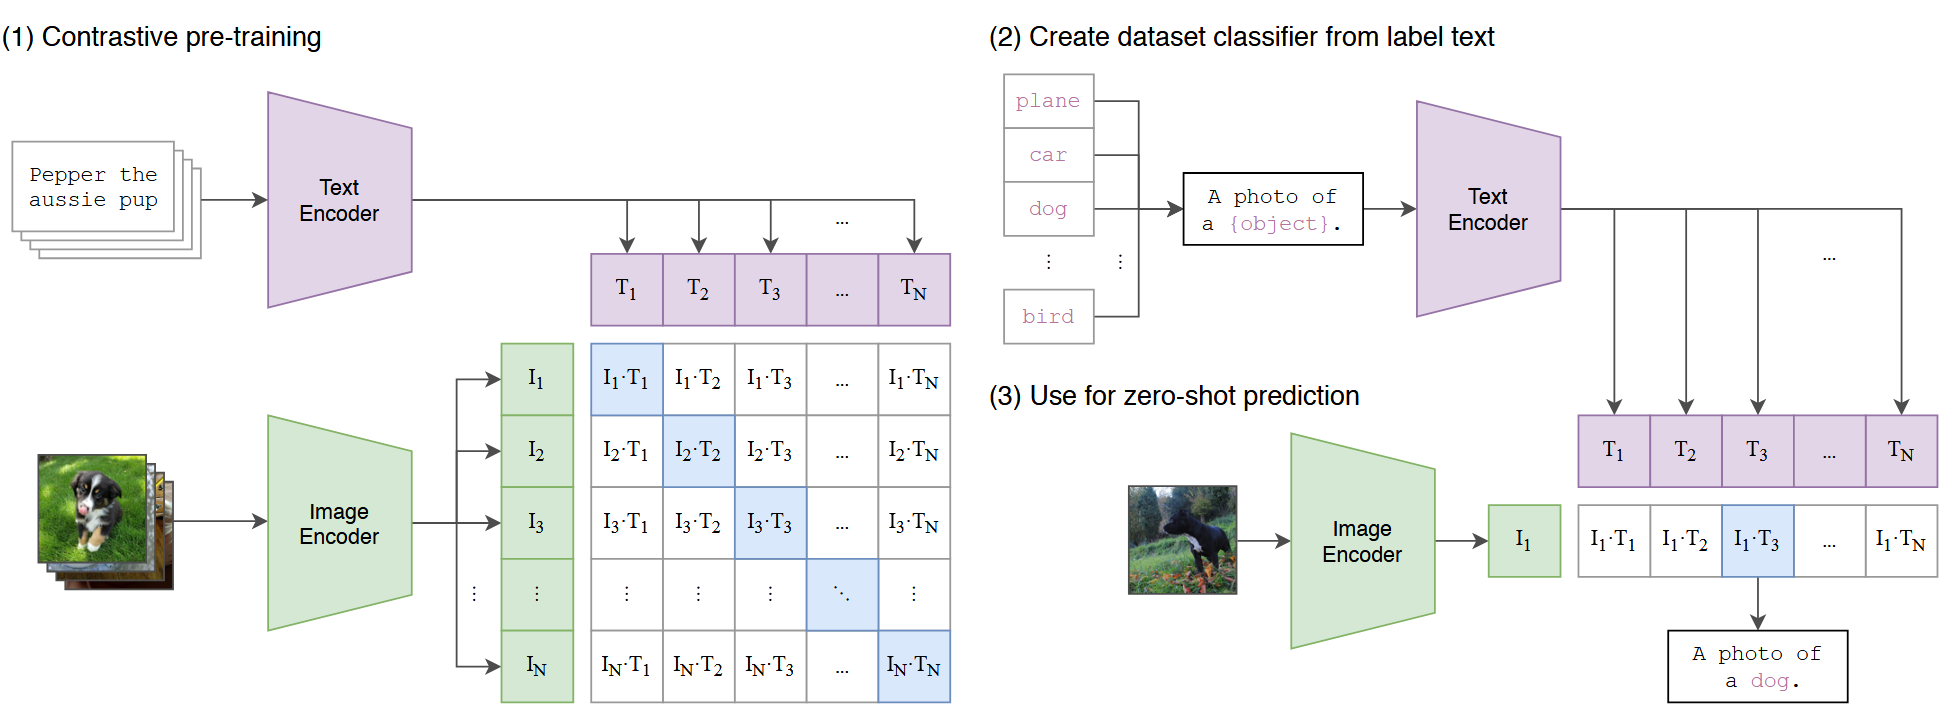
\includegraphics[width=0.8\linewidth]{clip.png}
    \caption[]{\scriptsize OpenAI CLIP ViT 总结~\parencite{radfordLearningTransferableVisual2021}。}
  \end{figure}
  \bottomleftrefs
\end{frame}
\end{refsection}



%--- 部分:数据增强 ---
\begin{refsection}
\begin{frame}
  \centering
  \vspace{2.5cm}
  {\LARGE \textbf{我们如何改进图像分类?}\\[0.5em]
  \textbf{(数据增强)}}
\end{frame}
\end{refsection}

%--- 数据增强:为什么? ---
\begin{refsection}
\begin{frame}{为什么要用数据增强?}
  \begin{minipage}{0.48\linewidth}
    \begin{itemize}
      \item 有时我们没有足够的图片来训练一个好的模型。
      \item 数据增强意味着用已有图片生成新的图片。
      \item 它能帮助模型学得更好,减少错误。
    \end{itemize}
  \end{minipage}%
  \hfill
  \begin{minipage}{0.48\linewidth}
    \centering
    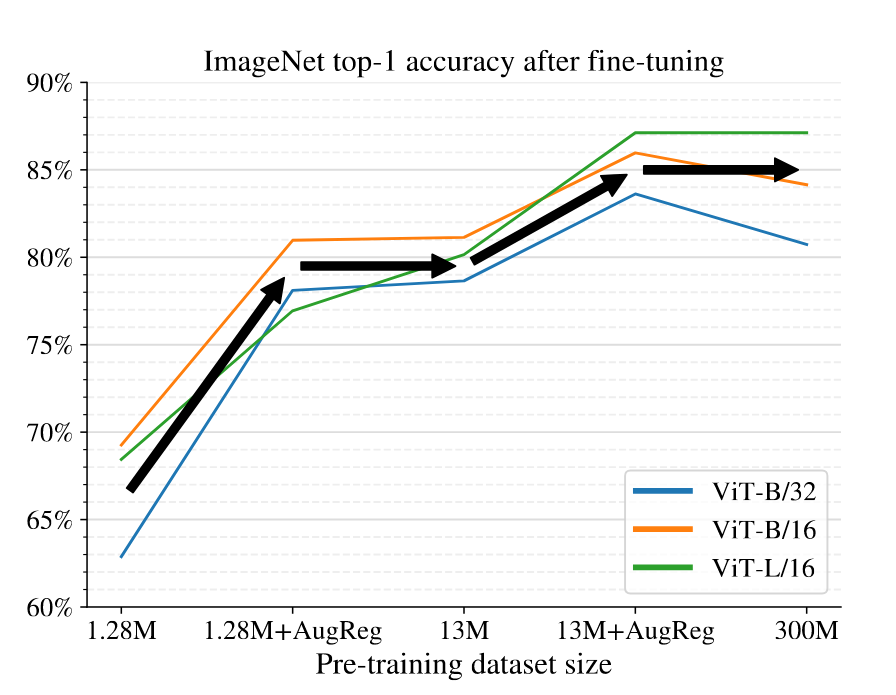
\includegraphics[width=0.95\linewidth]{augreg.png}
    \scriptsize \\
    图:适当的正则化和图像增强可以带来与数据集扩大十倍相似的提升效果。~\parencite{steinerHowTrainYour2022}
  \end{minipage}
  \bottomleftrefs
\end{frame}
\end{refsection}

%--- 数据增强:怎么做? ---
\begin{refsection}
\begin{frame}{我们如何进行数据增强?}
  \textbf{经典方法:}
  \begin{itemize}
    \item 翻转、旋转、裁剪、改变颜色等。
  \end{itemize}
  \textbf{现代方法:}
  \begin{itemize}
    \item 混合两张图片(Mixup)~\parencite{zhangMixupEMPIRICALRISK2018}。
    \item 剪切并粘贴图片部分(CutMix)~\parencite{yunCutMixRegularizationStrategy2019}。
  \end{itemize}
  \begin{figure}
    \centering
    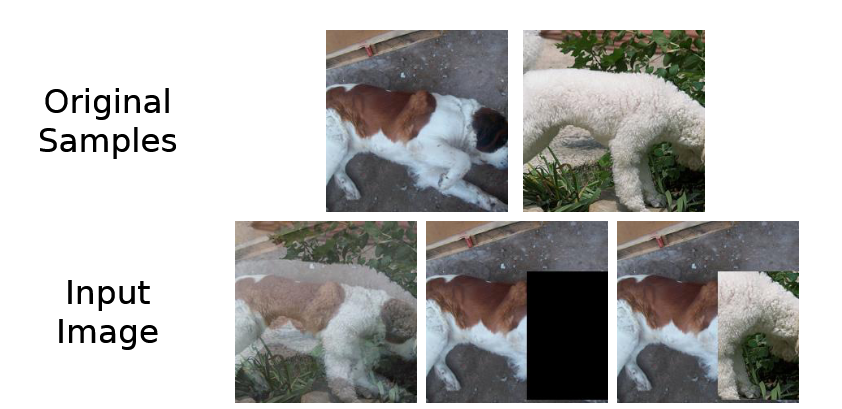
\includegraphics[width=0.5\linewidth]{aug_new_methods.png}
    \caption[]{\scriptsize 现代增强方法示意图。从左到右:Mixup~\parencite{zhangMixupEMPIRICALRISK2018},Cutout~\parencite{devriesImprovedRegularizationConvolutional2017},CutMix~\parencite{yunCutMixRegularizationStrategy2019}。}
  \end{figure}
  \bottomleftrefs
\end{frame}
\end{refsection}

%--- 示例数据集:RESISC45 ---
% \begin{refsection}
%   \begin{frame}{示例数据集:RESISC45}
%     \centering
%     \begin{figure}
%       \centering
%       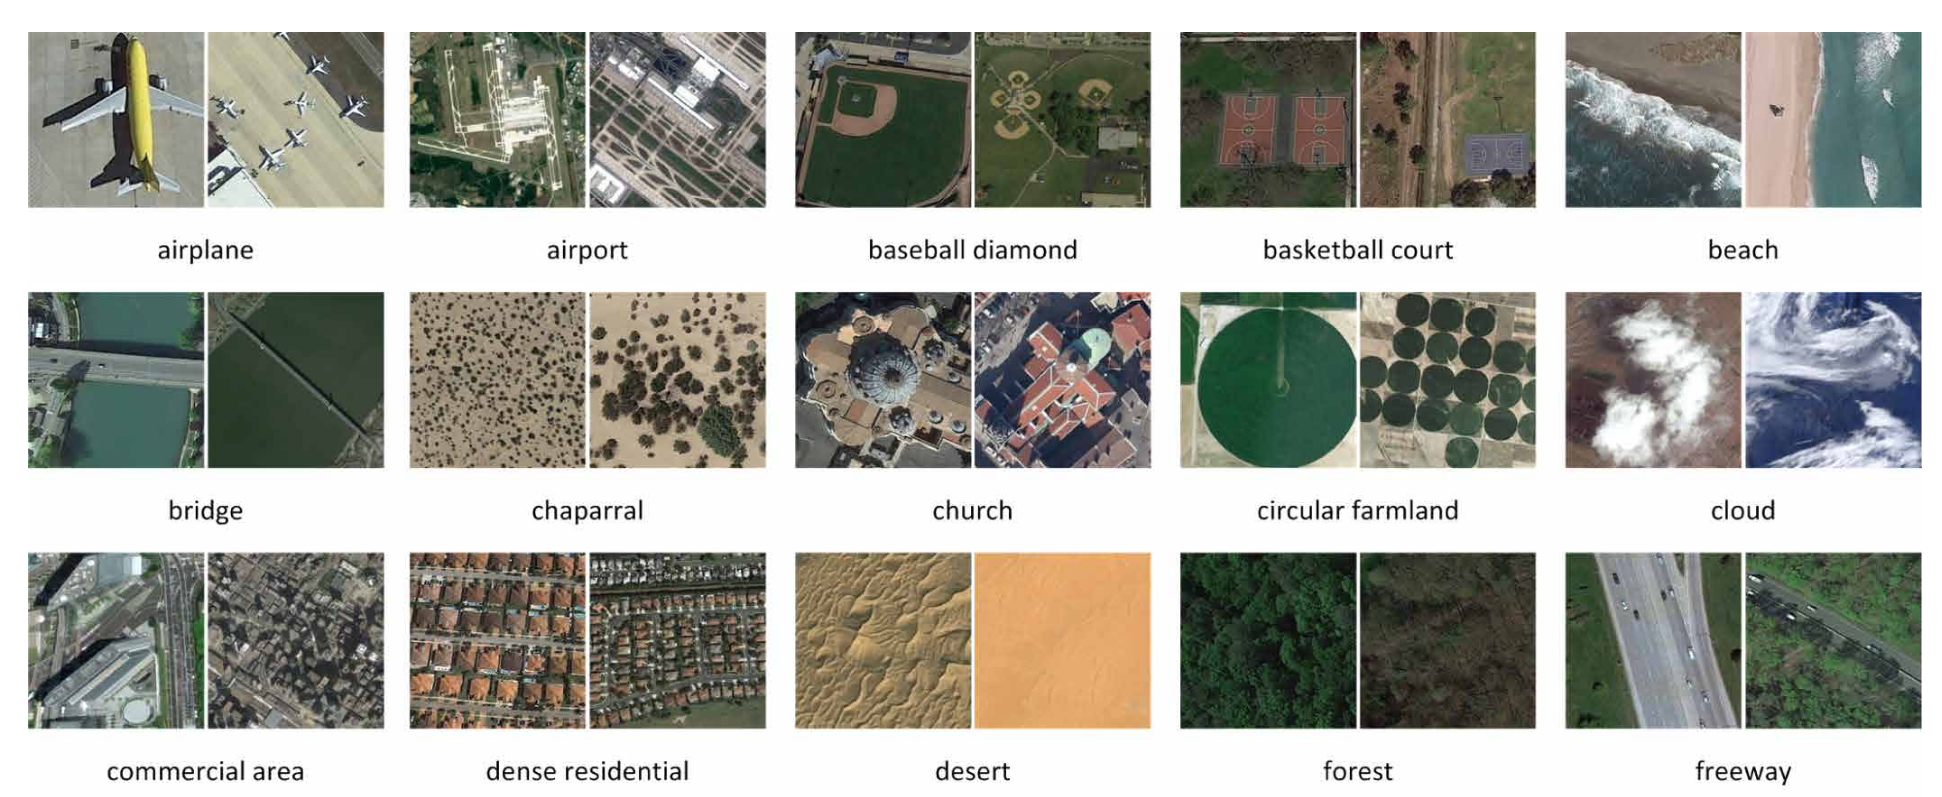
\includegraphics[width=1.0\linewidth]{RESISC45_part2.png}
%       \caption[]{\scriptsize RESISC45数据集示例图片~\parencite{Cheng2017},包含45个场景类别,每类700张图片。}
%     \end{figure}
%     \bottomleftrefs
%   \end{frame}
%   \end{refsection}

%--- 生成式模型用于数据增强 ---
\begin{refsection}
\begin{frame}{用生成式AI制作新图片}
  \begin{itemize}
    \item 生成式模型可以创造新的、逼真的图片。
    \item 我们可以用它们来生成更多训练数据。
    \item 例如:给一张“前”图片和描述,生成一张新的“后”图片。
  \end{itemize}
  \centering
  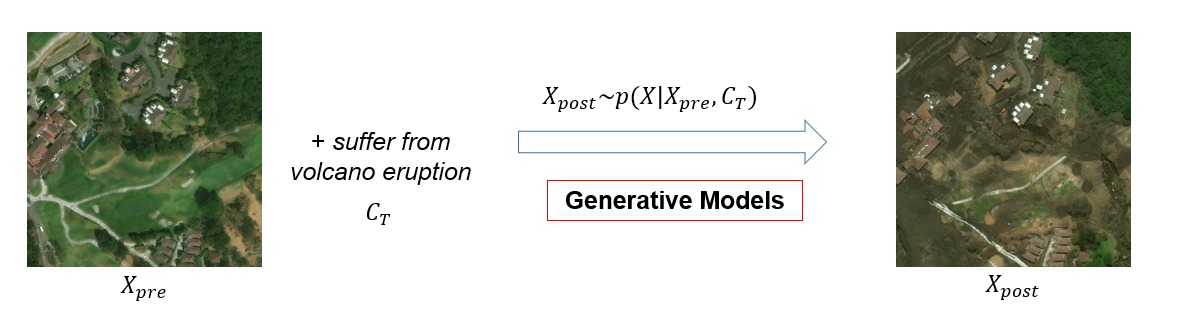
\includegraphics[width=1.0\linewidth]{diffusion_editing.png}
\end{frame}
\end{refsection}

%--- 真实案例:灾害图像(xBD) ---
\begin{frame}
  \centering
  \vspace{2.5cm}
  {\LARGE \textbf{真实案例:灾害图像(xBD)}}
\end{frame}

\begin{refsection}
  \begin{frame}{xBD:大规模灾害损失数据集}
    \begin{minipage}{0.42\linewidth}
      \centering
      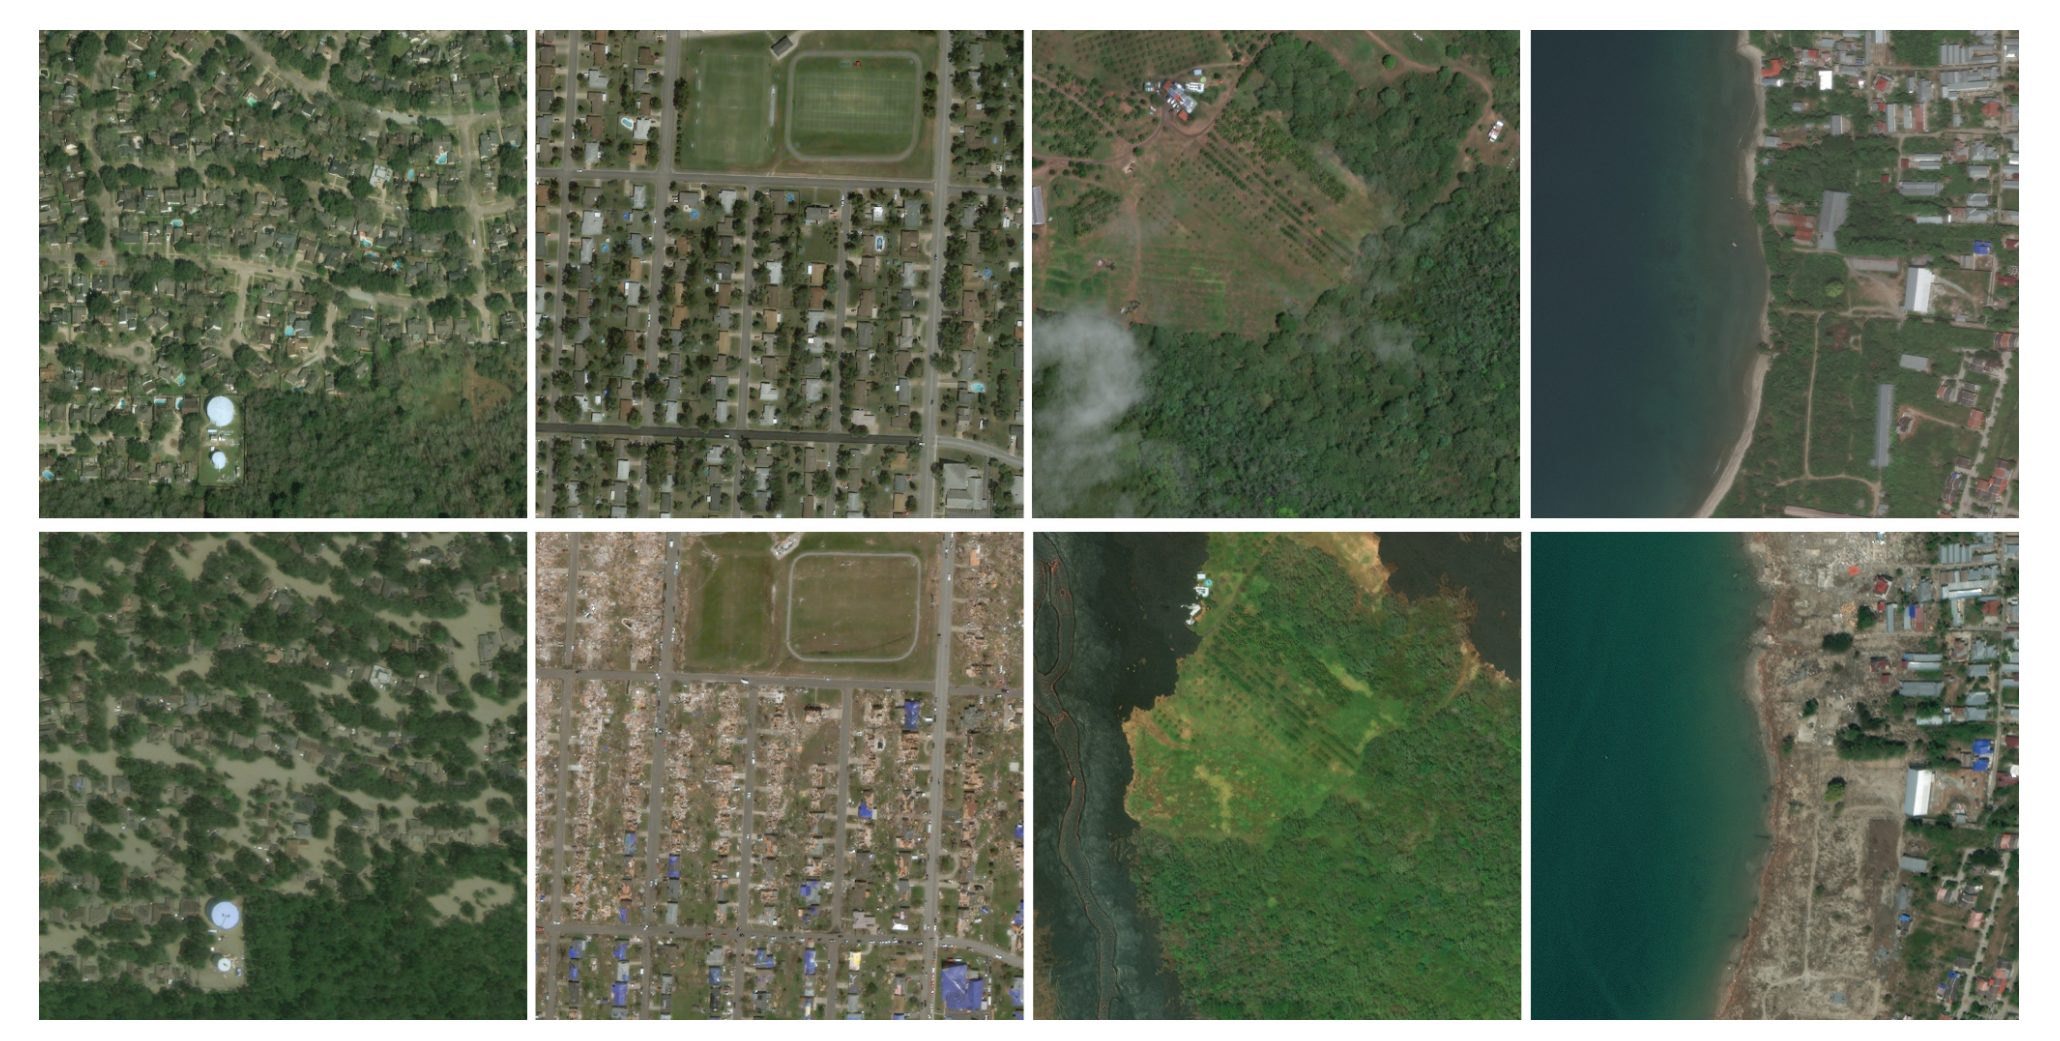
\includegraphics[width=1.0\linewidth]{xbd_samples.png}
      \vspace{0.5em}
      \scriptsize
      \textbf{xBD}~\parencite{guptaCreatingXBDDataset2019} 是一个双时相遥感数据集,涵盖19种不同的灾害事件。上方为灾前影像,下方为灾后影像。从左到右依次为:哈维飓风、乔普林龙卷风、Lower Puna火山喷发、巽他海峡海啸。
    \end{minipage}%
    \hfill
    \begin{minipage}{0.55\linewidth}
      \tiny
      \centering
      \textbf{表:xBD中的19个灾害事件。}
      \begin{tabular}{lll}
        \hline
        \textbf{灾害类型} & \textbf{灾害事件} & \textbf{事件日期} \\
        \hline
        地震 & 墨西哥城地震 & 2017年9月19日 \\
        森林火灾 & 葡萄牙森林火灾 & 2017年6月17--24日 \\
        森林火灾 & 圣罗莎森林火灾 & 2017年10月8--31日 \\
        森林火灾 & 卡尔森林火灾 & 2018年7月23--8月30日 \\
        森林火灾 & 伍尔西火灾 & 2018年11月9--28日 \\
        森林火灾 & 皮纳火灾 & 2018年11月25--12月2日 \\
        火山 & Lower Puna火山喷发 & 2018年5月23--8月14日 \\
        火山 & 危地马拉富埃戈火山喷发 & 2018年6月3日 \\
        风暴 & 阿拉巴马州塔斯卡卢萨龙卷风 & 2011年4月27日 \\
        风暴 & 密苏里州乔普林龙卷风 & 2011年5月22日 \\
        风暴 & 俄克拉荷马州穆尔龙卷风 & 2013年5月20日 \\
        风暴 & 马修飓风 & 2016年9月28--10月10日 \\
        风暴 & 佛罗伦萨飓风 & 2018年9月10--19日 \\
        洪水 & 尼泊尔、印度、孟加拉国季风 & 2017年8月 \\
        洪水 & 哈维飓风 & 2017年8月17--9月7日 \\
        洪水 & 迈克尔飓风 & 2018年10月7--16日 \\
        洪水 & 美国中西部洪水 & 2019年1月3--5月31日 \\
        海啸 & 印度尼西亚海啸 & 2018年9月18日 \\
        海啸 & 巽他海峡海啸 & 2018年12月22日 \\
        \hline
      \end{tabular}
      \vspace{0.5em}

    \end{minipage}
    \bottomleftrefs
  \end{frame}
\end{refsection}

%--- 项目部分 ---
\begin{frame}
  \centering
  \vspace{2.5cm}
  {\LARGE \textbf{项目:AI生成的图像能帮忙吗?}}
\end{frame}

%--- 项目:你会做什么? ---
\begin{refsection}
\begin{frame}{项目:你会做什么?}
  \begin{itemize}
    \item 测试加入AI生成图片是否能帮助模型学习。
    \item 尝试三种方式:
      \begin{itemize}
        \item 只用真实图片
        \item 只用生成图片
        \item 真实图片和生成图片混合
      \end{itemize}
    \item 看哪种方式效果最好!
  \end{itemize}
\end{frame}
\end{refsection}

%--- 项目:数据集与图片生成 ---
\begin{refsection}
\begin{frame}{项目:数据集细节与如何生成图片}
  \begin{itemize}
    \item 每种灾害类型使用100张真实图片(共6类,600张图片)。
    \item 每类用AI生成100–400张新图片。
    \item 尝试不同配比:1:1、1:2、1:3、1:4(真实:生成)。
    \item 使用商用AI模型(如GPT-Image-1~\parencite{gptimage1}、Gemini 2.5 Pro~\parencite{geminiteamgoogleGemini25Pushing}、SeedEdit 3.0~\parencite{wang2025seedit})生成图片。
    \item 输入:一张“前”图片和简短描述(如“让它遭受洪水”)。
    \item 输出:一张新的、逼真的“后”图片。
  \end{itemize}
  \bottomleftrefs
\end{frame}
\end{refsection}

%--- 项目:模型与评估 ---
\begin{refsection}
\begin{frame}{用哪些模型与如何衡量效果}
  \begin{itemize}
    \item \textbf{尝试这些模型:}
      \begin{itemize}
        \item OpenAI CLIP~\parencite{radfordLearningTransferableVisual2021}
        \item Google SigLip/SigLip2~\parencite{tschannenSigLIP2Multilingual2025,Zhai_2023_ICCV}
        \item 以上模型均采用ViT结构(见\href{https://github.com/huggingface/transformers/blob/main/examples/pytorch/contrastive-image-text/README.md}{\textcolor{blue}{CLIP训练示例}}和\href{https://github.com/NielsRogge/Transformers-Tutorials/tree/master/VisionTransformer}{\textcolor{blue}{ViT教程}})。
      \end{itemize}
    \item \textbf{如何衡量效果:}
      \begin{itemize}
        \item \textbf{准确率}:正确答案的百分比
        \item \textbf{F1分数}:平衡精确率和召回率
        \item \textbf{混淆矩阵}:展示哪些类别容易混淆
      \end{itemize}
    \item 始终在模型未见过的真实图片上测试。
    \item 用简单的柱状图或折线图对比结果。
  \end{itemize}
  \bottomleftrefs
\end{frame}
\end{refsection}